\section{Overview}

This section gives an overview of our attacking system which exploits Deep Learning techniques to recognize current Captchas. The system takes in a distorted text-based Captcha with complex noisy background. It automatically generated the regular Captcha corresponding to the distorted one. At last, the regular Captcha is cracked by CNN recognition engine. Figure~\ref{fig:overview} depicts the three steps of our attack:

\begin{figure}
  \centering
  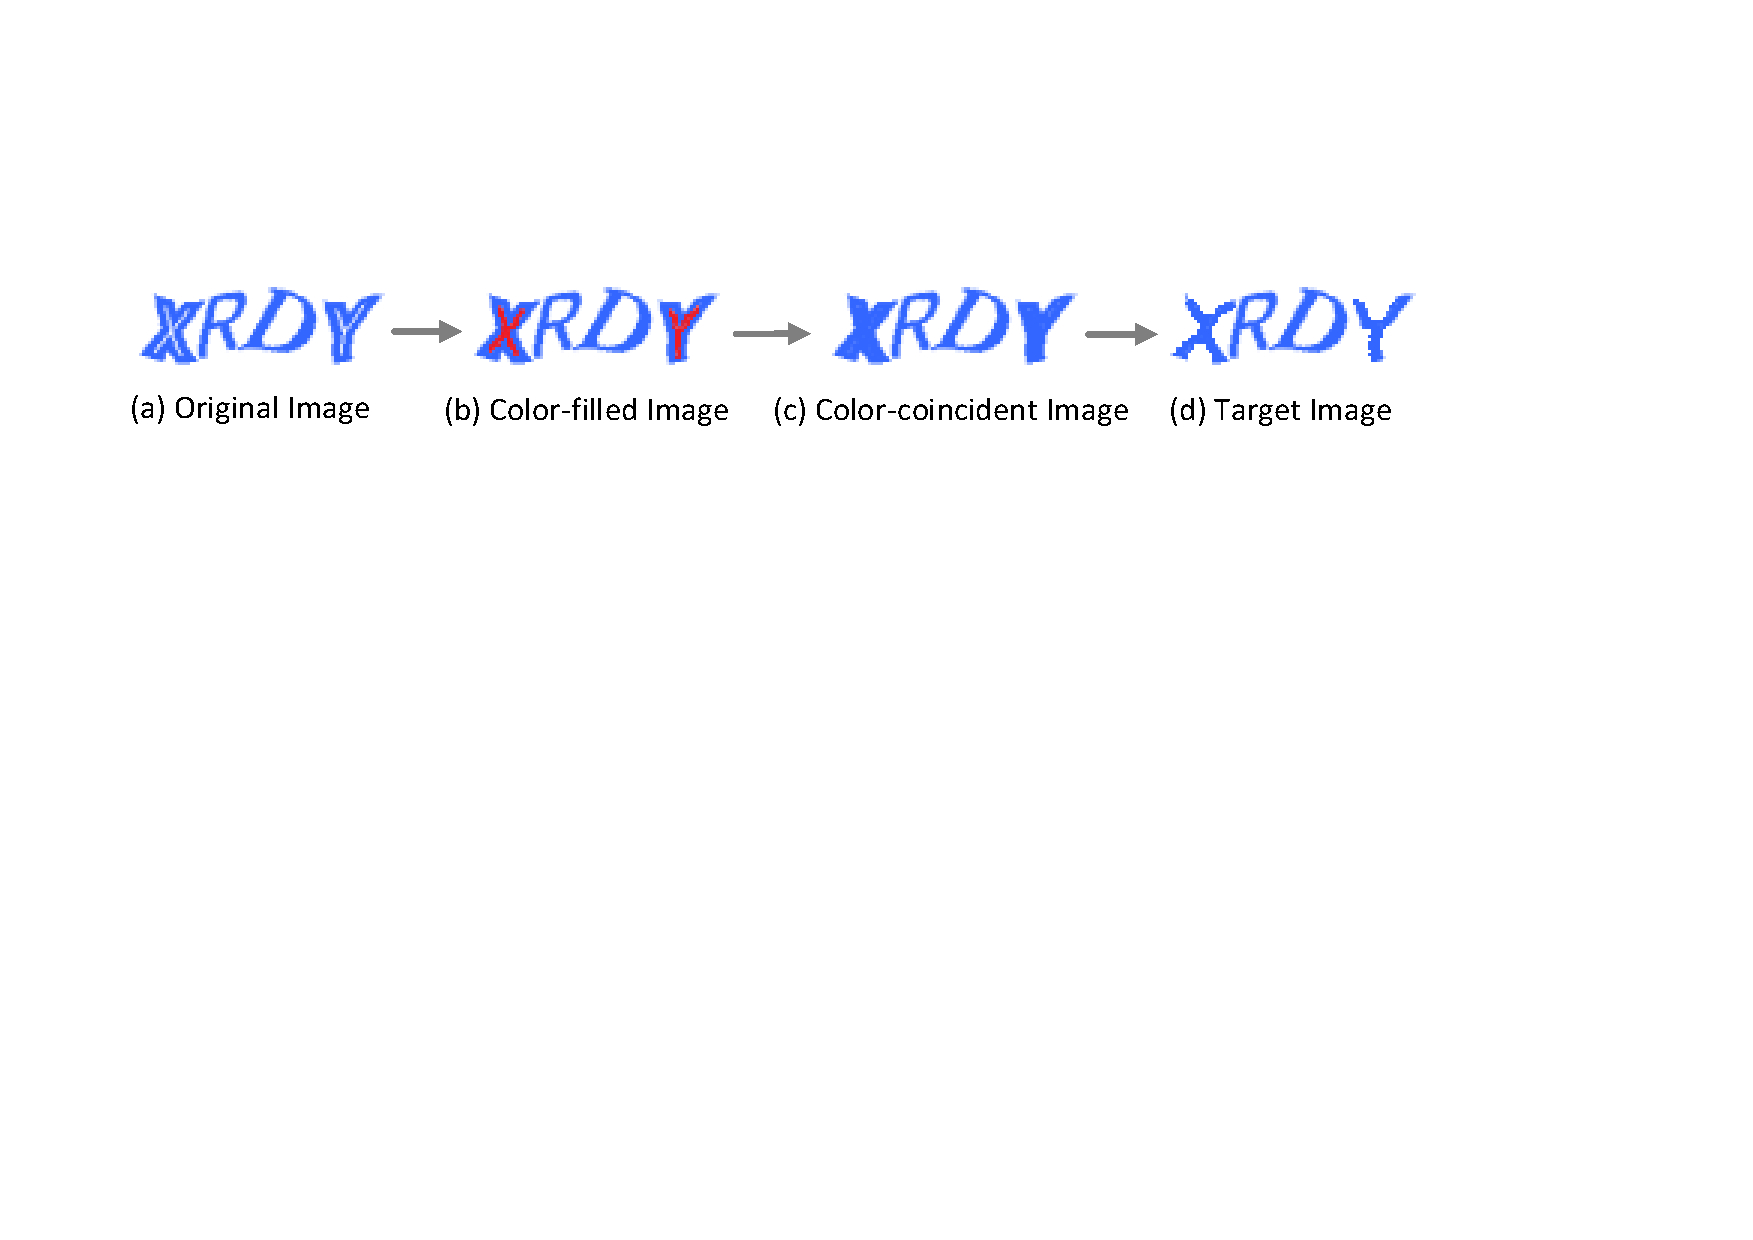
\includegraphics[width=0.5\textwidth]{fig/fill_color.pdf}
  \caption{The procedure of Captcha preprocessing.}
  \label{fig:fill_color}
\end{figure}

\noindent \textbf{\emph{Step 1. Captcha Preprocessing}}

The attack begins from inputting the distorted Captchas with complex background and overlapping characters. Given the characters on Captcha have different styles (see Figure~\ref{fig:fill_color} (a), it includes both hollow and solid characters), it is necessary to uniform the style of these characters for further processing. We have shown that the system can automatically translate the hollow character to the solid one (Figure~\ref{fig:fill_color}).

\noindent \textbf{\emph{Step 2. Generate Regular Captcha}}

Once the style of character on Captcha image is uniformed, a deep learning algorithm will be applied to generate the regular Captcha shown as Figure~\ref{fig:overview}. We archive this through hierarchical approaches described as the following three steps:

\noindent \circling{\textcolor{white}{1}} \textbf{Remove Noisy Background:}  To generate the regular Captcha, the first step is to clean the complex background, and produce the Captcha with white background.
To do so, a deep learning algorithm will be applied to remove the complex noisy background stay on Captcha.
For each Captcha scheme, this algorithm needs to train the model for cleaning our the background.

\noindent \circling{\textcolor{white}{2}} \textbf{Expand Space Between Adjacent Characters:} This step aims to increase the distance between two characters on Captcha. We use the same algorithm as step 2 to enlarge the inter-character distance and generate a new Captcha. Keep in mind that the Captcha generated at this stage is distorted.

\noindent \circling{\textcolor{white}{3}} \textbf{Regularization:} In this step, our system is able to automatically translate the distorted Captcha to a regular one.

\noindent \textbf{\emph{Step 3. Recognize Captcha}}

In this final step, we use a radical CNN model as the recognition engine to identify the text of the regular Captcha translated from last step.



